\subsection{Đăng ký - Đăng nhập}
\subsubsection{Sơ đồ use-case}
\begin{figure}[H]
    \centering
    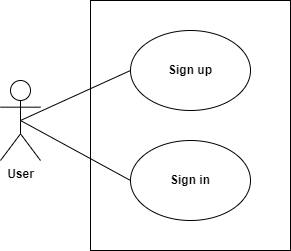
\includegraphics[width=0.4\textwidth]{Images/UseCase/Auth.png}
    \caption{Sơ đồ use-case cho chức năng đăng nhập và đăng ký}
\end{figure}
\newpage
\subsubsection{Đặc tả use-case cho chức năng đăng ký tài khoản}
\begin{center}
    \arrayrulecolor{cyan!75!black}
    \arrayrulewidth=2pt
    \begin{longtable}{
        |>{\raggedright\arraybackslash}p{3cm}
        |>{\raggedright\arraybackslash}p{13cm}
        |}
        \hline
        \rowcolor{cyan!75!black} \textcolor{white}{\textbf{Use-case name}} & \textcolor{white}{\textbf{ĐĂNG KÝ}}
        \\\hline
        \rowcolor{cyan!10!white} \textit{Actor} & Người dùng
        \\\hdashline
        \rowcolor{cyan!10!white} \textit{Description} & Người dùng tạo tài khoản với email và mật khẩu, sau đó người dùng có thể sử dụng tài khoản này để đăng nhập vào ứng dụng. 
        \\\hdashline
        \rowcolor{cyan!10!white} \textit{Preconditions} & Không có
        \\\hdashline
        \rowcolor{cyan!10!white} \textit{Postconditions} & Người dùng đăng ký tài khoản thành công. Người dùng có thể sử dụng tài khoản này để truy cập vào ứng dụng
        \\\hdashline
        \rowcolor{cyan!10!white} \textit{Trigger} & Người dùng nhấn chọn vào nút \textbf{Đăng ký} ở giao diện ứng dụng.
        \\\hdashline
        \rowcolor{cyan!10!white} \textit{Main flow} & 
        1. Ứng dụng hiển thị trang đăng ký và yêu cầu người dùng nhập các thông tin cần thiết để tạo tài khoản. \newline
        2. Người dùng nhập trường thông tin để tạo tài khoản. \newline
        3. Người dùng nhấn nút \textbf{Đăng ký}. \newline
        4. Ứng dụng xác minh thông tin đã nhập và tạo tài khoản mới. \newline
        5. Ứng dụng thông báo đăng ký tài khoản thành công.
        \\\hdashline
        \rowcolor{cyan!10!white} \textit{Alternative flow} & 
        \textbf{Nếu người dùng hủy đăng ký tài khoản, ứng dụng sẽ quay trở lại giao diện chính} \newline
        2a.1. Người dùng hủy quá trình đăng ký tài khoản. \newline
        2a.2. Ứng dụng quay trở lại giao diện chính.
        \\\hdashline
        \rowcolor{cyan!10!white} \textit{Exception flow} & 
        \textbf{Nếu thông tin đăng ký không được cung cấp đầy đủ, ứng dụng sẽ hiển thị lỗi và yêu cầu người dùng cung cấp lại thông tin} \newline
        4a.1. Ứng dụng thông báo thông tin đăng ký chưa đầy đủ. \newline
        4a.2. Người dùng bổ sung thông tin đăng ký. \newline
        4a.3. Ứng dụng kiểm tra thông tin đã nhập. \newline
        4a.4. Nếu thông tin hợp lệ, ứng dụng sẽ thông báo đăng ký tài khoản thành công, ngược lại sẽ quay lại bước 2. \newline
        \textbf{Nếu thông tin đăng ký không hợp lệ, ứng dụng sẽ hiển thị lỗi và yêu cầu người dùng cung cấp lại thông tin} \newline
        4a.1. Ứng dụng thông báo thông tin đăng ký không hợp lệ. \newline
        4a.2. Người dùng chỉnh sửa thông tin đăng ký. \newline
        4a.3. Ứng dụng kiểm tra thông tin đã nhập. \newline
        4a.4. Nếu thông tin hợp lệ, ứng dụng sẽ thông báo đăng ký tài khoản thành công, ngược lại sẽ quay lại bước 2. \newline
        \textbf{Nếu người dùng đã có tài khoản trên ứng dụng, ứng dụng sẽ báo lỗi và yêu cầu người dùng đăng ký bằng tài khoản khác} \newline
        4b.1. Ứng dụng thông báo tài khoản đã tồn tại. \newline
        4b.2. Người dùng nhập lại tài khoản. \newline
        4b.3. Ứng dụng kiểm tra thông tin đăng ký đã nhập. \newline
        4b.4. Nếu thông tin hợp lệ, ứng dụng sẽ thông báo đăng ký tài khoản thành công, ngược lại sẽ quay lại bước 2. \newline
        \textbf{Nếu ứng dụng gặp lỗi trong quá trình đăng ký tài khoản, ứng dụng thông báo lỗi và yêu cầu người dùng thử lại sau} \newline
        4c.1. Ứng dụng hiện lỗi khi xác minh thông tin đăng ký. \newline
        4c.2. Ứng dụng thông báo yêu cầu người dùng thử lại sau. 
        \\\hline
        \caption{Đặc tả use-case cho chức năng đăng ký tài khoản}
    \end{longtable}
\end{center}
\subsubsection{Đặc tả use-case cho chức năng đăng nhập}
\begin{center}
    \arrayrulecolor{cyan!75!black}
    \arrayrulewidth=2pt
    \begin{longtable}{
        |>{\raggedright\arraybackslash}p{3cm}
        |>{\raggedright\arraybackslash}p{13cm}
        |}
        \hline
        \rowcolor{cyan!75!black} \textcolor{white}{\textbf{Use-case name}} & \textcolor{white}{\textbf{ĐĂNG NHẬP}}
        \\\hline
        \rowcolor{cyan!10!white} \textit{Actor} & Người dùng
        \\\hdashline
        \rowcolor{cyan!10!white} \textit{Description} & Tính năng đăng nhập cho phép người dùng đăng nhập vào ứng dụng bằng tên đăng nhập và mật khẩu của họ. Nếu thông tin đăng nhập chính xác, họ có thể sử dụng các tính năng chính trong ứng dụng.
        \\\hdashline
        \rowcolor{cyan!10!white} \textit{Preconditions} & Người dùng cần có tài khoản đã đăng ký trên ứng dụng.
        \\\hdashline
        \rowcolor{cyan!10!white} \textit{Postconditions} & Người dùng được đăng nhập vào ứng dụng và có thể truy cập vào các tính năng chính trong ứng dụng.
        \\\hdashline
        \rowcolor{cyan!10!white} \textit{Trigger} & Người dùng nhấn chọn vào nút \textbf{Đăng nhập} ở giao diện ứng dụng.
        \\\hdashline
        \rowcolor{cyan!10!white} \textit{Main flow} & 
        1. Ứng dụng hiển thị trang đăng nhập và yêu cầu người dùng nhập tên đăng nhập và mật khẩu. \newline
        2. Người dùng nhập thông tin tài khoản của mình vào các trường tương ứng. \newline
        3. Người dùng nhấn nút \textbf{Đăng nhập}. \newline
        4. Ứng dụng xác minh thông tin đăng nhập. \newline
        5. Ứng dụng thông báo đăng nhập thành công.
        \\\hdashline
        \rowcolor{cyan!10!white} \textit{Alternative flow} & 
        \textbf{Nếu người dùng hủy đăng nhập tài khoản, ứng dụng sẽ quay trở lại giao diện chính} \newline
        2a.1. Người dùng hủy quá trình đăng ký tài khoản. \newline
        2a.2. Ứng dụng quay trở lại giao diện chính.
        \\\hdashline
        \rowcolor{cyan!10!white} \textit{Exception flow} & 
        \textbf{Nếu thông tin đăng nhập không được cung cấp đầy đủ, ứng dụng sẽ hiển thị lỗi và yêu cầu người dùng cung cấp lại thông tin} \newline
        4a.1. Ứng dụng thông báo thông tin đăng nhập chưa đầy đủ. \newline
        4a.2. Người dùng bổ sung thông tin đăng nhập. \newline
        4a.3. Ứng dụng kiểm tra thông tin đã nhập. \newline
        4a.4. Nếu thông tin hợp lệ, ứng dụng sẽ thông báo đăng nhập tài khoản thành công, ngược lại sẽ quay lại bước 2. \newline
        \textbf{Nếu thông tin đăng nhập không hợp lệ, ứng dụng sẽ hiển thị lỗi và yêu cầu người dùng cung cấp lại thông tin} \newline
        4a.1. Ứng dụng thông báo thông tin đăng nhập không hợp lệ. \newline
        4a.2. Người dùng chỉnh sửa thông tin đăng nhập. \newline
        4a.3. Ứng dụng kiểm tra thông tin đã nhập. \newline
        4a.4. Nếu thông tin hợp lệ, ứng dụng sẽ thông báo đăng nhập tài khoản thành công, ngược lại sẽ quay lại bước 2. \newline
        \textbf{Nếu người dùng chưa có tài khoản trên ứng dụng, ứng dụng sẽ báo lỗi và yêu cầu người dùng phải sử dụng tài khoản đã đăng ký để đăng nhập} \newline
        4b.1. Ứng dụng thông báo tài khoản chưa tồn tại. \newline
        4b.2. Người dùng nhập lại tài khoản. \newline
        4b.3. Ứng dụng kiểm tra thông tin đăng nhập đã nhập. \newline
        4b.4. Nếu thông tin hợp lệ, ứng dụng sẽ thông báo đăng nhập tài khoản thành công, ngược lại sẽ quay lại bước 2. \newline
        \textbf{Nếu ứng dụng gặp lỗi trong quá trình đăng nhập tài khoản, ứng dụng thông báo lỗi và yêu cầu người dùng thử lại sau} \newline
        4c.1. Ứng dụng hiện lỗi khi xác minh thông tin đăng nhập. \newline
        4c.2. Ứng dụng thông báo yêu cầu người dùng thử lại sau.
        \\\hline
        \caption{Đặc tả use-case cho chức năng đăng nhập tài khoản}
    \end{longtable}
\end{center}
